\documentclass[border=10pt]{standalone}

\usepackage{xcolor}

% --- Definiciones de color de la figura ---

% Opción 1: Usando códigos Hex (HTML)
\definecolor{miAzul}{HTML}{6688AA}
\definecolor{miNaranja}{HTML}{DDAA44}
\definecolor{miVerde}{HTML}{88BB44}
\definecolor{miMorado}{HTML}{884488}

\usepackage{physics}

\usepackage{graphicx}
\graphicspath{
  {/home/jadeleon/Documents/chaos_meets_channels/ja_files/figs_ja/choi/purity_dynamics/}
  {/home/jadeleon/Documents/chaos_meets_channels/ja_files/figs_ja/bloch/}
  {/home/jadeleon/Documents/chaos_meets_channels/ja_files/figs_ja/}
  {/home/jadeleon/Documents/doctorado/2025-2/protocolo_candidatura/gfx/chaos/}
}
\usepackage{tikz}

\begin{document}
\fontsize{10}{10}\selectfont
\begin{tikzpicture}
% Definir separación
\def\sep{-0.2cm}

% Figura izquierda
\node[anchor=north west] (fig1) at (0,0) 
    {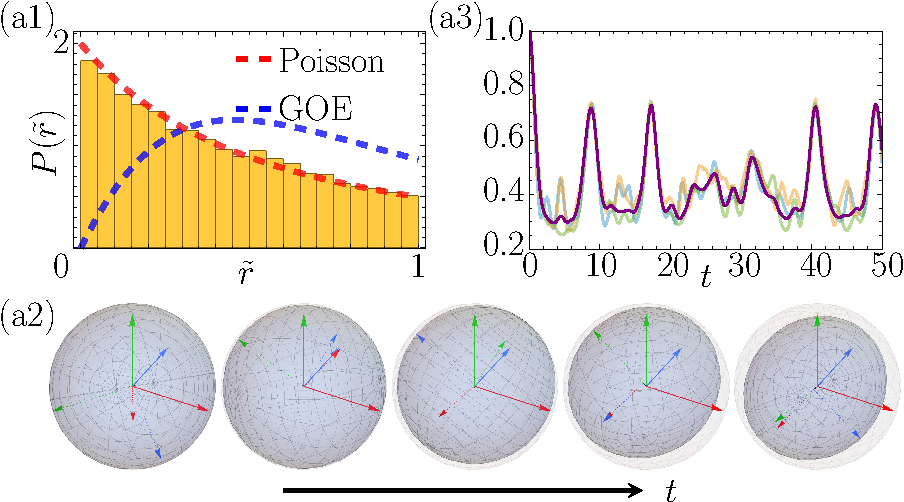
\includegraphics[width=0.48\textwidth]{cj_purity_regular.pdf}};

% Figura derecha
\node[anchor=north west] (fig2) at ([xshift=\sep]fig1.north east) 
    {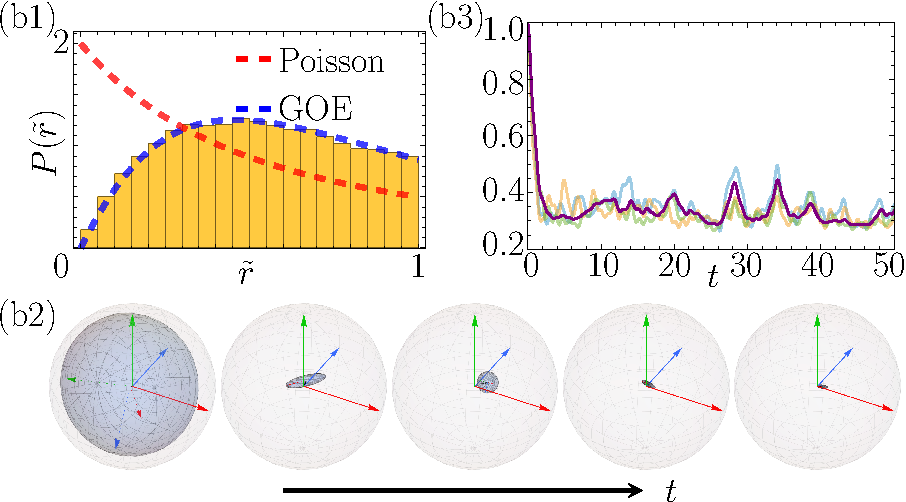
\includegraphics[width=0.48\textwidth]{cj_purity_chaotic.pdf}};

\begin{scope}[shift={([xshift=-3.2cm, yshift=0.05cm]fig1.north east)}, local bounding box=leyendas]
% Tres líneas horizontales una sobre otra
\draw[miAzul, line width=0.4pt, opacity=0.75] (0,0.07) -- (0.5,0.07); % Línea arriba

\draw[miNaranja, line width=0.4pt, opacity=0.75] (0,0) -- (0.5,0);
\node[pos=1, anchor=west, xshift=15pt, scale=0.65, black] at (0.5,0)
    {Single realizations of $\Tr[\mathcal{D}(t)^2]$};


\draw[miVerde, line width=0.4pt, opacity=0.75] (0,-0.07) -- (0.5,-0.07); % Línea abajo

% Línea morada a la derecha de las otras
\draw[miMorado, line width=0.9pt, opacity=1.] ([xshift=0.1cm]leyendas.east) -- 
    ([xshift=0.5cm]leyendas.east)
    node[pos=1, anchor=west, xshift=1pt, scale=0.65, black] {$\ev{\Tr[\mathcal{D}(t)^2]}_{\mathrm{Haar}}$};
\end{scope}
\end{tikzpicture}
\end{document}